\chapter{Implementation of Graph Representation}
\label{graphimplementationappendix}
In the following python code there is the implementation for the all the different graph representation, and the operation of insertion of nodes and edges.

\begin{lstlisting}[firstnumber=1, caption={Graph representation and fundamental operations.}]
class Node():

	def __init__(self, value):
		self.value = value
		self.edges = []

class Edge():

	def __init__(self, value, node_from, node_to):
		self.value = value
		self.node_from = node_from
		self.node_to = node_to
		
class Graph():
	
	def __init__(self, nodes=[], edges=[]):
		self.nodes = nodes
		self.edges = edges
	
	def insert_node(self, new_node_value):
		new_node = Node(new_node_value)
		self.nodes.append(new_node)
		
	def insert_edge(self, new_edge_val, node_from, val, node_to_val):
		from_found = None
		for node in self.nodes:
			if node_from_val == node.value:
				from_found = node
			if node_to_val == node.value:
				to_found = node
			if from_found == None:
				from_found = node(node_from_val=
				self.nodes.append(from_found)
			if to_found == None:
				to_found = Node(node_to_val)
				self.nodes.append(to_found)
		new_edge = Edge(new_edge_val, from_found, to_found)
		from_found.edges.append(new_edge)
		to_found.edges.append(new_edge)
		self.edges.append(new_edge)
	
	def get_edge_list(self):
		get_list = []
		for edge_object in self.edges:
			edge = (edge_object.value, edge_object.node_from_value.value, edge_object.node_to.value)
			edge_list.append(edge)
		return edge_list
	
	def get_adjacency_list(self):
		max_index = self.find_max_index()
		dajacency_list = [None]*(max_index + 1)
		for edge_object in self.edges:
			if adjacency_list[edge_object.node_from.value]:
				adjacency_list[edge_object.node_from.value].append((edge_object.node_to.value, edge_object.value))
			else:
				adjacency_list[edge_object.node_from.value] = [(edge_object.node_to.value, edge_object.value)]
		return adjacency_list
		
	def get_adjacency_matrix(self):
		max_index = self.find_max_inde()
		adjacency_matrix = [[0 for i in range(max_index + 1)] for j in range(max_index + 1)]
		for edge_object in self.edges:
			adjacency_matrix[edge_object.node_from.value][edge_object.node_to.value] = edge_object.value
		return adjacency_matrix
		
	def find_max_index(self):
		max_index = 1
		if len(self.node):
			for node in self.nodes:
				if node.value > max_index:
					max_index = node.value
		return max_index
\end{lstlisting}

\chapter{Implementation of Graph Traversal}
\label{graphimplementationtraversalappendix}
In the following chapter \textbf{depth-first search} and \textbf{breadth-first search} are implemented, with both recursive and iterative implementation.
\section{Depth-first search}
In the following there are the pesudocode, the python implementation, and an example of execution of the depth-first search on a graph.

\begin{algorithm}[H]
	\DontPrintSemicolon
	\LinesNumbered
  	\SetKwFunction{FIterativeDepthFirstSearch}{Iterative-Depth-first-search}
  	\SetKwFunction{FRecursiveDepthFirstSearch}{Recursive-Depth-first-search}
  	\SetKwProg{Fn}{Function}{:}{}
  	\Fn{\FRecursiveDepthFirstSearch{$graph$, $vertex$}}{
  		visit(vertex)\;
  		\For{\normalfont{all adjacent nodes adj\textunderscore vertices to vertex}}{
			\FRecursiveDepthFirstSearch{$graph$, $adj_vertices$}\;		
  		}
  	}
  	\;
  	\Fn{\FIterativeDepthFirstSearch{$graph$, $vertex$}}{
		s $\leftarrow$ \textbf{empty stack}\;
		s.push(vertex)\;
		\While{\normalfont{\textbf{not} s.isEmpty()}}{
			vertex $\leftarrow$ s.pop()\;
			\If{\normalfont{vertex \textbf{not} visited}}{
				visit(vertex)\;
				\For{\normalfont{all adjacent nodes adj\textunderscore vertices to vertex}}{
					s.push(adj\textunderscore vertices)\;
				}
			}
		}  	
  	}
\caption{Depth-first search pseudocode.}
\end{algorithm}

\begin{lstlisting}[firstnumber=1, caption={Recursive and iterative implementation of depth-first search on graphs.}]
		
class Graph():
	...
	
	def depth_first_search_recursive(self, start_node):
		ret_list = [start_node]
		start_node.visited = True
		edges_out = [e for e in start_node.edges
					 if e.node_to.value != start_node.value]
		for e in edges_out:
			if not edge.node.visited:
				ret_list.extend(
					depth_first_search_recursive(
						
	
\end{lstlisting}

\begin{figure}[H]
	\begin{center}
		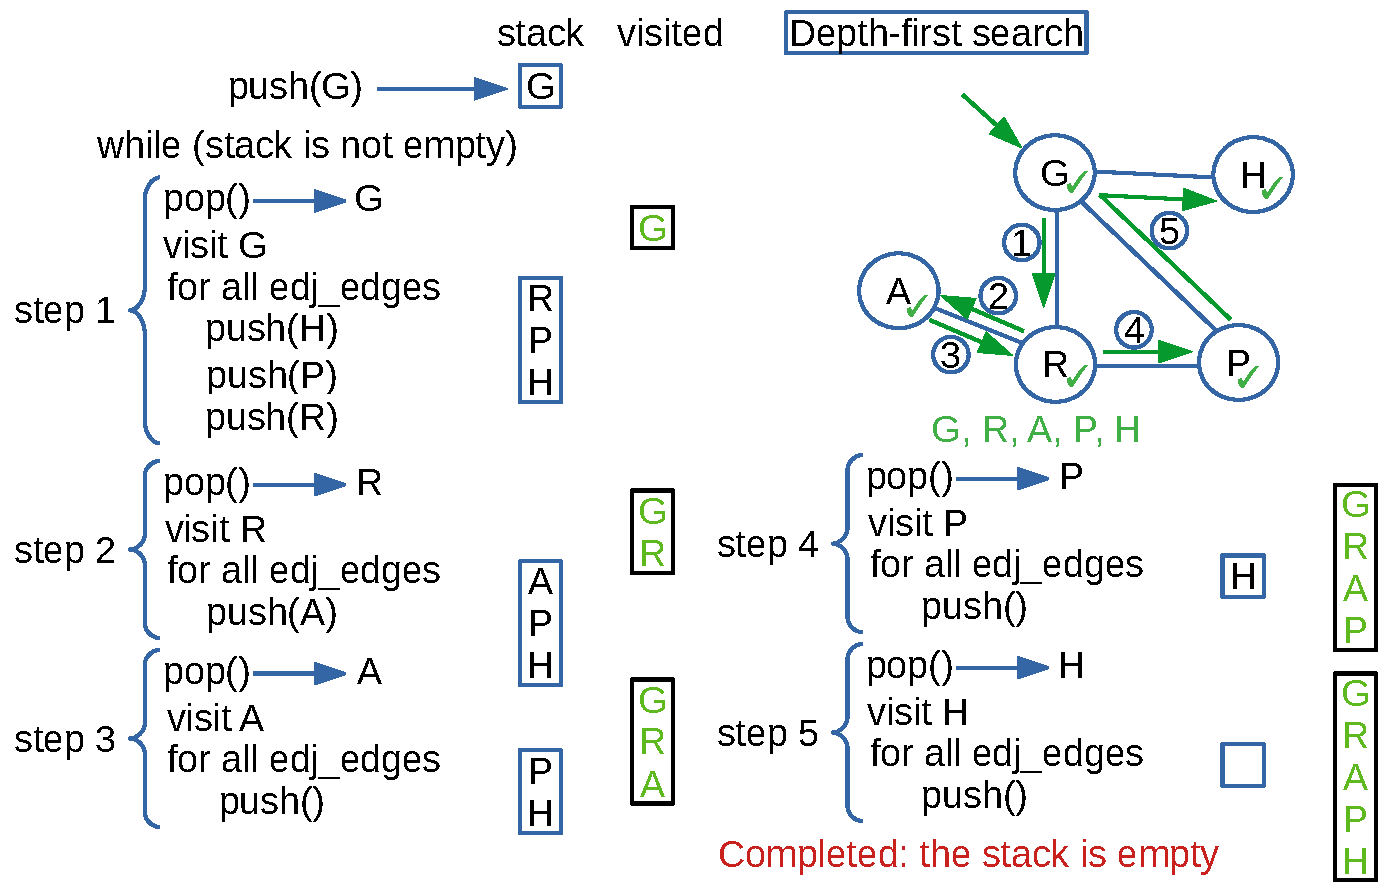
\includegraphics[scale=.6]{chapters/appendix/images/appendixgraphs/graphsappendix_1.pdf}
		\caption[Depth-first search example.]{Depth-first search example.}
		\label{graphappendix_1}
	\end{center}
\end{figure}

\begin{figure}[H]
\centering
\begin{tikzpicture} [node distance={15mm}, thick, main/.style = {draw, circle, minimum size=8mm}]  
  
  \node[main] (na) at (0,0) {$a$};
  \node[main] (nb) at (2,0) {$b$};
  \node[main] (nc) at (2,-2) {$c$};
  \node[main] (nd) at (0,-2) {$d$};
  \node[main] (ne) at (-2,-1.8) {$e$};
  
  \draw (na) -- (nb);
  \draw (na) -- (nc);
  \draw (na) -- (nd);
  \draw (nd) -- (nc);
  \draw (nd) -- (ne);
  
  \draw[->, >=stealth, BrickRed] ($(na) + (-0.7,0.7)$) -- (na);
  \path[->, BrickRed, >=stealth] (na.west) edge [bend right=20] node[draw=none, xshift=-4pt] {1} (nd.north west);
  \path[->, BrickRed, >=stealth] (nd.north west) edge [bend right=20] node[draw=none, yshift=4pt] {2} (ne.north east);
  \path[->, BrickRed, >=stealth] (ne.south east) edge [bend right=20] node[draw=none, yshift=-5pt] {} (nd.south west);
  \path[->, BrickRed, >=stealth] (nd.south east) edge [bend right=20] node[draw=none, yshift=-5pt] {3} (nc.south west);
  \path[BrickRed] (nc.north) edge [bend right=20] node[draw=none, xshift=4pt, yshift=4pt] {4} (na.south east);
  \path[->, BrickRed, >=stealth] (na.south east) edge [bend right=20] node[draw=none, yshift=4pt] {} (nb.south west);
  
  \draw ($(na) + (-2.6, 0.4)$) node[rectangle] {Depth-first search};
  \draw ($(nd) + (-0.5,-1)$) node[align=left] {a, d, e, c, b};
  
% Stack 1
\draw ($(na) + (4, 0.4)$) node[draw=none, rectangle, align=left] (stack) {Stack};

\draw[-] ($(stack.west) + (0,-4mm)$) -- ($(stack.west) + (0,-20mm)$);
\draw[-] ($(stack.west) + (10mm,-4mm)$) -- ($(stack.west) + (10mm,-20mm)$);
\draw[-] ($(stack.west) + (0,-20mm)$) -- ($(stack.west) + (10mm,-20mm)$);
\draw ($(stack.south) + (-1mm,-13.5mm)$) node[draw, rectangle, rounded corners, minimum width=0.5cm, minimum height=0.5cm] (a1) {a};
\draw ($(stack.south) + (0,-22mm)$) node[draw, rectangle, minimum width=0.6cm, minimum height=0.6cm] (visited) {\textcolor{ForestGreen}{a}};
\path[->, >=stealth] ($(a1.north west) + (-10mm,3mm)$) edge [bend left=20] node[draw=none, xshift=-6pt, yshift=-7pt] {push} (a1.north west);
\path[->, >=stealth] (a1.north) edge [bend left=20] node[draw=none, xshift=-4pt, yshift=7pt] {pop} ($(a1.north east) + (1mm, 5mm)$);

% Stack 2
\draw ($(stack) + (1, 0)$) node[draw=none, rectangle, align=left] (stack1) {};
\draw[-] ($(stack1.west) + (0,-4mm)$) -- ($(stack1.west) + (0,-20mm)$);
\draw[-] ($(stack1.west) + (10mm,-4mm)$) -- ($(stack1.west) + (10mm,-20mm)$);
\draw[-] ($(stack1.west) + (0,-20mm)$) -- ($(stack1.west) + (10mm,-20mm)$);
\draw ($(stack1.south) + (3.5mm,-15mm)$) node[draw, rectangle, rounded corners, minimum width=0.5cm, minimum height=0.5cm] (b2) {b};
\draw ($(stack1.south) + (3.5mm,-9mm)$) node[draw, rectangle, rounded corners, minimum width=0.5cm, minimum height=0.5cm] (c2) {c};
\draw ($(stack1.south) + (3.5mm,-3mm)$) node[draw, rectangle, rounded corners, minimum width=0.5cm, minimum height=0.5cm] (d2) {d};
\draw[->, >=stealth] (a1.east) -- (b2.west);
\draw[->, >=stealth] (a1.east) -- (c2.west);
\draw[->, >=stealth] (a1.east) -- (d2.west);
\draw ($(visited.east) + (10mm,0)$) node[draw, rectangle, minimum width=0.6cm, minimum height=0.6cm] {\textcolor{ForestGreen}{a, d}};

% Stack 3
\draw ($(stack1) + (1.5, 0)$) node[draw=none, rectangle, align=left] (stack2) {};
\draw[-] ($(stack2.west) + (0,-4mm)$) -- ($(stack2.west) + (0,-20mm)$);
\draw[-] ($(stack2.west) + (10mm,-4mm)$) -- ($(stack2.west) + (10mm,-20mm)$);
\draw[-] ($(stack2.west) + (0,-20mm)$) -- ($(stack2.west) + (10mm,-20mm)$);
\draw ($(stack2.south) + (3.5mm,-15mm)$) node[draw, rectangle, rounded corners, minimum width=0.5cm, minimum height=0.5cm] (b3) {b};
\draw ($(stack2.south) + (3.5mm,-9mm)$) node[draw, rectangle, rounded corners, minimum width=0.5cm, minimum height=0.5cm] (c3) {c};
\draw ($(stack2.south) + (3.5mm,-3mm)$) node[draw, rectangle, rounded corners, minimum width=0.5cm, minimum height=0.5cm] (e3) {e};
\draw[->, >=stealth] (d2.east) -- (e3.west);
\draw ($(visited.east) + (25mm,0)$) node[draw, rectangle, minimum width=0.6cm, minimum height=0.6cm] {\textcolor{ForestGreen}{a, d, e}};

% Stack 4
\draw ($(stack2) + (1.5, 0)$) node[draw=none, rectangle, align=left] (stack3) {};
\draw[-] ($(stack3.west) + (0,-4mm)$) -- ($(stack3.west) + (0,-20mm)$);
\draw[-] ($(stack3.west) + (10mm,-4mm)$) -- ($(stack3.west) + (10mm,-20mm)$);
\draw[-] ($(stack3.west) + (0,-20mm)$) -- ($(stack3.west) + (10mm,-20mm)$);
\draw ($(stack3.south) + (3.5mm,-15mm)$) node[draw, rectangle, rounded corners, minimum width=0.5cm, minimum height=0.5cm] (b4) {b};
\draw ($(stack3.south) + (3.5mm,-9mm)$) node[draw, rectangle, rounded corners, minimum width=0.5cm, minimum height=0.5cm] (c4) {c};
\draw ($(visited.east) + (44mm,0)$) node[draw, rectangle, minimum width=0.6cm, minimum height=0.6cm] {\textcolor{ForestGreen}{a, d, e, c}};

% Stack 5
\draw ($(stack) + (-0.45, -2.5)$) node[draw=none, rectangle, align=left] (stack4) {};
\draw[-] ($(stack4.west) + (0,-4mm)$) -- ($(stack4.west) + (0,-20mm)$);
\draw[-] ($(stack4.west) + (10mm,-4mm)$) -- ($(stack4.west) + (10mm,-20mm)$);
\draw[-] ($(stack4.west) + (0,-20mm)$) -- ($(stack4.west) + (10mm,-20mm)$);
\draw ($(stack4.south) + (3.5mm,-15mm)$) node[draw, rectangle, rounded corners, minimum width=0.5cm, minimum height=0.5cm] (b5) {b};
\draw ($(stack4.south) + (1mm,-23mm)$) node[draw, rectangle, minimum width=0.6cm, minimum height=0.6cm] {\textcolor{ForestGreen}{a, d, e, c, b}};

% Stack 6
\draw ($(stack4) + (1.45, 0)$) node[draw=none, rectangle, align=left] (stack5) {};
\draw[-] ($(stack5.west) + (0,-4mm)$) -- ($(stack5.west) + (0,-20mm)$);
\draw[-] ($(stack5.west) + (10mm,-4mm)$) -- ($(stack5.west) + (10mm,-20mm)$);
\draw[-] ($(stack5.west) + (0,-20mm)$) -- ($(stack5.west) + (10mm,-20mm)$);
\draw ($(stack5.east) + (20mm,-10mm)$) node[draw=none, rectangle, minimum width=0.6cm, minimum height=0.6cm] {\textcolor{BrickRed}{Stack empty}}; 

\end{tikzpicture}
\caption[Depth-first search example.]{Depth-first search example.}
\label{graphappendix_1}
\end{figure}

\section{Breadth-first search}
In the following there are the pesudocode, the python implementation, and an example of execution of the breadth-first search on a graph.

\begin{algorithm}[H]
	\DontPrintSemicolon
	\LinesNumbered
  	\SetKwFunction{FBreadthFirstSearch}{Breadth-first-search}
  	\SetKwProg{Fn}{Function}{:}{}
  	\Fn{\FBreadthFirstSearch{$graph$, $vertex$}}{
		q $\leftarrow$ \textbf{empty queue}\;
		visit(vertex)\;
		q.enqueue(vertex)\;
		\While{\normalfont{\textbf{not} q.isEmpty()}}{
			vertex $\leftarrow$ s.dequeue()\;
			\For{\normalfont{all adjacent nodes adj\textunderscore vertices to vertex}}{
				\If{\normalfont{adj\textunderscore \textbf{not} visited}}{
					visit(adj\textunderscore vertices)\;
					q.enqueue(adj\textunderscore vertices)\;
				}
			}
		}  	
  	}
\caption{Breadth-first search pseudocode.}
\end{algorithm}

\begin{lstlisting}[firstnumber=1, caption={Breadth-first search implementation on graphs.}]
		
class Graph():
	...
	
	def breadth_first_search(self, start_node):
		ret_list = [start_node]
		start_node.visited = True
		edges_out = [e for e in start_node.edges
					 if e.node_to.value != start_node.value]
		for e in edges_out:
			if not edge.node.visited:
				ret_list.extend(
					depth_first_search_recursive(
						
	
\end{lstlisting}

\begin{figure}[H]
	\begin{center}
		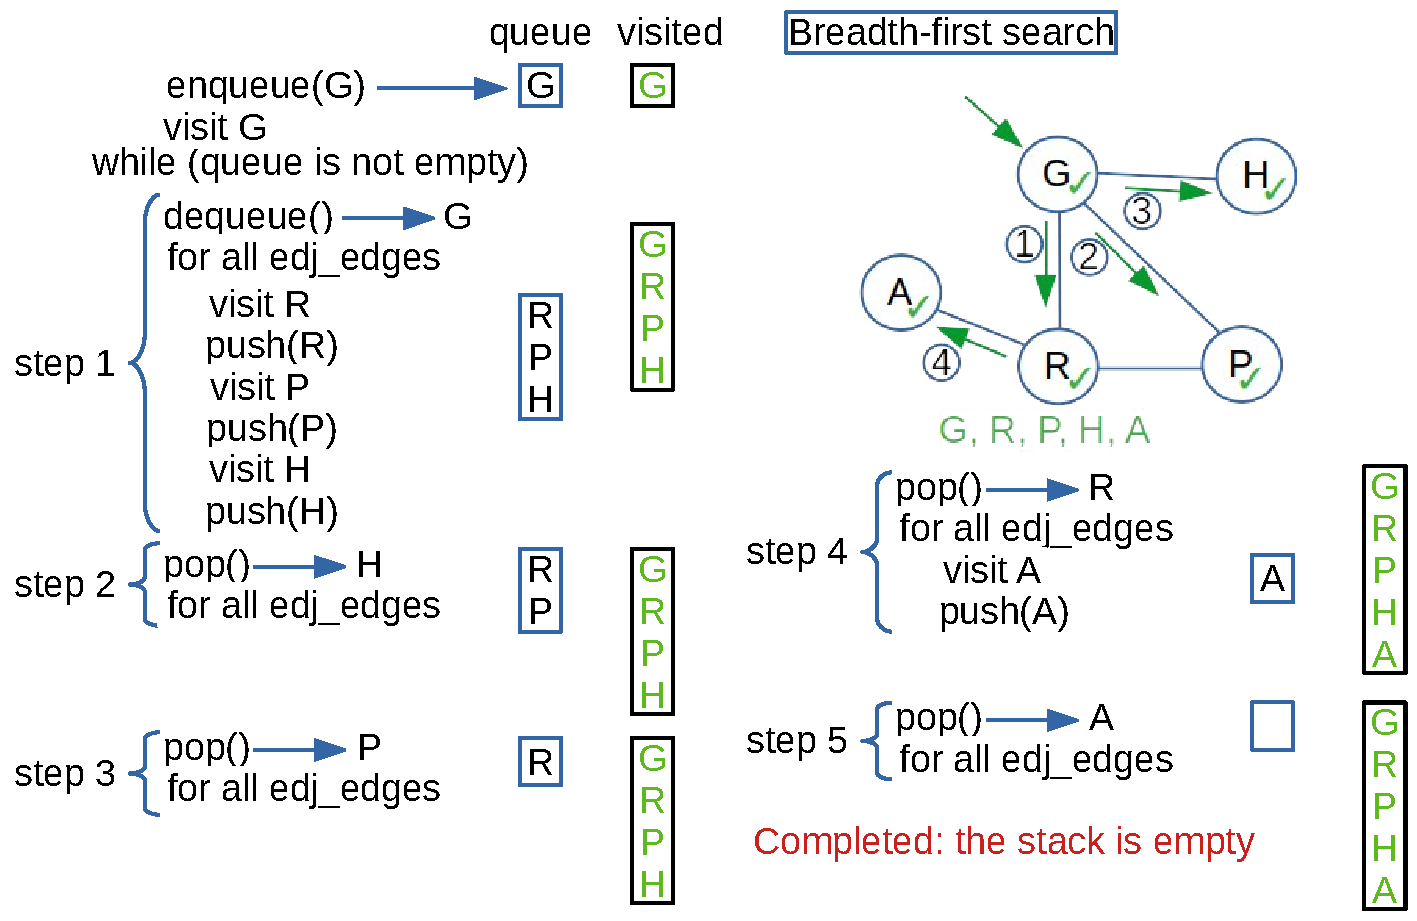
\includegraphics[scale=.6]{chapters/appendix/images/appendixgraphs/graphsappendix_2.pdf}
		\caption[Breadth-first search example.]{Breadth-first search example.}
		\label{graphappendix_2}
	\end{center}
\end{figure}

\begin{figure}[H]
\centering
\begin{tikzpicture} [node distance={15mm}, thick, main/.style = {draw, circle, minimum size=8mm}]  
  
  \node[main] (na) at (0,0) {$a$};
  \node[main] (nb) at (2,0) {$b$};
  \node[main] (nc) at (2,-2) {$c$};
  \node[main] (nd) at (0,-2) {$d$};
  \node[main] (ne) at (-2,-1.8) {$e$};
  
  \draw (na) -- (nb);
  \draw (na) -- (nc);
  \draw (na) -- (nd);
  \draw (nd) -- (nc);
  \draw (nd) -- (ne);
  
  \draw[->, >=stealth, BrickRed] ($(na) + (-0.7,0.7)$) -- (na);
  \path[->, BrickRed, >=stealth] (na.west) edge [bend right=20] node[draw=none, xshift=-4pt] {1} (nd.north west);
  \path[->, BrickRed, >=stealth] (na.south) edge [bend right=30] node[draw=none, xshift=-4pt, yshift=-4pt] {2} (nc.north west);
  \path[->, BrickRed, >=stealth] (na.north east) edge [bend left=20] node[draw=none, yshift=5pt] {3} (nb.north west);
  \path[->, BrickRed, >=stealth] (nd.south west) edge [bend left=20] node[draw=none, yshift=-5pt] {4} (ne.south east);
  
  \draw ($(na) + (-2.6, 0.4)$) node[rectangle] {Breadth-first search};
  \draw ($(nd) + (-0.5,-1)$) node[align=left] {a, d, c, b, e};
  
% Queue 1
\draw ($(na) + (4, 0.4)$) node[draw=none, rectangle, align=left] (queue) {Queue};

\draw[-] ($(queue.west) + (0,-4mm)$) -- ($(queue.west) + (0,-20mm)$);
\draw[-] ($(queue.west) + (10mm,-4mm)$) -- ($(queue.west) + (10mm,-20mm)$);
\draw ($(queue.south) + (-2.5mm,-13.5mm)$) node[draw, rectangle, rounded corners, minimum width=0.5cm, minimum height=0.5cm] (a1) {a};
\draw ($(queue.south) + (0,-22mm)$) node[draw, rectangle, minimum width=0.6cm, minimum height=0.6cm] (visited) {\textcolor{ForestGreen}{a}};
\path[->, >=stealth] ($(a1.north west) + (-10mm,3mm)$) edge [bend left=20] node[draw=none, xshift=-6pt, yshift=-7pt] {enq} (a1.north west);
\path[->, >=stealth] (a1.south west) edge [bend left=20] node[draw=none, xshift=-6pt, yshift=7pt] {deq} ($(a1.north east) + (-15mm, -10mm)$);

% queue 2
\draw ($(queue) + (1, 0)$) node[draw=none, rectangle, align=left] (queue1) {};
\draw[-] ($(queue1.west) + (0,-4mm)$) -- ($(queue1.west) + (0,-20mm)$);
\draw[-] ($(queue1.west) + (10mm,-4mm)$) -- ($(queue1.west) + (10mm,-20mm)$);
\draw ($(queue1.south) + (3.5mm,-15mm)$) node[draw, rectangle, rounded corners, minimum width=0.5cm, minimum height=0.5cm] (d2) {d};
\draw ($(queue1.south) + (3.5mm,-9mm)$) node[draw, rectangle, rounded corners, minimum width=0.5cm, minimum height=0.5cm] (c2) {c};
\draw ($(queue1.south) + (3.5mm,-3mm)$) node[draw, rectangle, rounded corners, minimum width=0.5cm, minimum height=0.5cm] (b2) {b};
\draw[->, >=stealth] (a1.east) -- (b2.west);
\draw[->, >=stealth] (a1.east) -- (c2.west);
\draw[->, >=stealth] (a1.east) -- (d2.west);
\draw ($(visited.east) + (10mm,0)$) node[draw, rectangle, minimum width=0.6cm, minimum height=0.6cm] {\textcolor{ForestGreen}{a, d}};

% queue 3
\draw ($(queue1) + (1.5, 0)$) node[draw=none, rectangle, align=left] (queue2) {};
\draw[-] ($(queue2.west) + (0,-4mm)$) -- ($(queue2.west) + (0,-20mm)$);
\draw[-] ($(queue2.west) + (10mm,-4mm)$) -- ($(queue2.west) + (10mm,-20mm)$);
\draw ($(queue2.south) + (3.5mm,-15mm)$) node[draw, rectangle, rounded corners, minimum width=0.5cm, minimum height=0.5cm] (c3) {c};
\draw ($(queue2.south) + (3.5mm,-9mm)$) node[draw, rectangle, rounded corners, minimum width=0.5cm, minimum height=0.5cm] (b3) {b};
\draw ($(visited.east) + (25mm,0)$) node[draw, rectangle, minimum width=0.6cm, minimum height=0.6cm] {\textcolor{ForestGreen}{a, d, c}};

% queue 4
\draw ($(queue2) + (1.5, 0)$) node[draw=none, rectangle, align=left] (queue3) {};
\draw[-] ($(queue3.west) + (0,-4mm)$) -- ($(queue3.west) + (0,-20mm)$);
\draw[-] ($(queue3.west) + (10mm,-4mm)$) -- ($(queue3.west) + (10mm,-20mm)$);
\draw ($(queue3.south) + (3.5mm,-15mm)$) node[draw, rectangle, rounded corners, minimum width=0.5cm, minimum height=0.5cm] (b4) {b};
\draw ($(visited.east) + (44mm,0)$) node[draw, rectangle, minimum width=0.6cm, minimum height=0.6cm] {\textcolor{ForestGreen}{a, d, c, b}};

% queue 5
\draw ($(queue) + (-0.45, -2.5)$) node[draw=none, rectangle, align=left] (queue4) {};
\draw[-] ($(queue4.west) + (0,-4mm)$) -- ($(queue4.west) + (0,-20mm)$);
\draw[-] ($(queue4.west) + (10mm,-4mm)$) -- ($(queue4.west) + (10mm,-20mm)$);
\draw ($(queue4.south) + (3.5mm,-15mm)$) node[draw, rectangle, rounded corners, minimum width=0.5cm, minimum height=0.5cm] (e5) {e};
\draw ($(queue4.south) + (1mm,-23mm)$) node[draw, rectangle, minimum width=0.6cm, minimum height=0.6cm] {\textcolor{ForestGreen}{a, d, c, b, e}};

% queue 6
\draw ($(queue4) + (1.45, 0)$) node[draw=none, rectangle, align=left] (queue5) {};
\draw[-] ($(queue5.west) + (0,-4mm)$) -- ($(queue5.west) + (0,-20mm)$);
\draw[-] ($(queue5.west) + (10mm,-4mm)$) -- ($(queue5.west) + (10mm,-20mm)$);
\draw ($(queue5.east) + (20mm,-10mm)$) node[draw=none, rectangle, minimum width=0.6cm, minimum height=0.6cm] {\textcolor{BrickRed}{queue empty}};
      
\end{tikzpicture}  
\caption[Breadth-first search example.]{Breadth-first search example.}
\label{graphappendix_2}
\end{figure}

\chapter{Complexity of Data Structures for Graphs}
\label{graphsappendix}
In the following table are summarized the complexities of the most common operations on graphs for the different data structures \cite{goodrich2013data}.

\chapter{Dijkstra's Algorithm Implementation}
\label{dijkstraimplementation}
As described in the section \ref{sec:dijkstra} the Dijkstra's algorithm is a greedy algorithm that find the optimal solution by finding the optimal solution at each step. The implementation of the Dijkstra's algorithm is based on priority queue.

Let us consider the following graph (Figure \ref{graphappendix_3}).

\begin{figure}[H]
	\begin{center}
		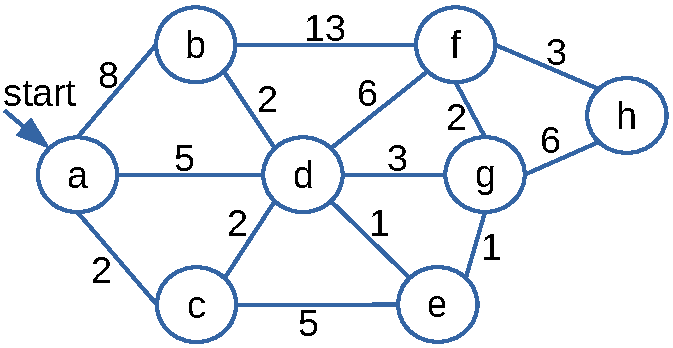
\includegraphics[scale=.6]{chapters/appendix/images/appendixgraphs/graphsappendix_3.pdf}
		\caption[Dijkstra's algorithms example.]{Dijkstra's algorithms example.}
		\label{graphappendix_3}
	\end{center}
\end{figure}

\begin{figure}[H]

\centering
\begin{tikzpicture}[node distance={15mm}, thick, main/.style = {draw, circle, minimum size=8mm}]

		\node[main] (nd) at (0,0) {d};
		\node[main] (na) at (-2.5,0) {a};
		\node[main] (nb) at (-1.5,1.5) {b};
		\node[main] (nc) at (-1.5,-1.5) {c};
		\node[main] (nf) at (1.5,1.5) {f};
		\node[main] (ne) at (1.5,-1.5) {e};
		\node[main] (ng) at (2.5,0) {g};
		\node[main] (nh) at (3.2,1.1) {h};
		
		\node[draw=none] (start) at ($(na) + (-1,1)$) {Start};
		
		\draw[->, >=stealth] (start) -- (na);
		
		\draw (na) edge node[draw=none, xshift=-6pt] {$8$} (nb);
		\draw (na) edge node[draw=none, xshift=-6pt] {$2$} (nc);
		\draw (na) edge node[draw=none, yshift=6pt] {$5$} (nd);
		\draw (nb) edge node[draw=none, xshift=6pt] {$2$} (nd);
		\draw (nb) edge node[draw=none, yshift=6pt] {$13$} (nf);
		\draw (nc) edge node[draw=none, xshift=-6pt] {$2$} (nd);
		\draw (nc) edge node[draw=none, yshift=-6pt] {$5$} (ne);
		\draw (nd) edge node[draw=none, xshift=-6pt] {$6$} (nf);
		\draw (nd) edge node[draw=none, yshift=7pt] {$3$} (ng);
		\draw (nd) edge node[draw=none, xshift=6pt] {$1$} (ne);
		\draw (ne) edge node[draw=none, xshift=-6pt] {$1$} (ng);
		\draw (nf) edge node[draw=none, xshift=6pt] {$2$} (ng);
		\draw (nf) edge node[draw=none, xshift=6pt, yshift=4pt] {$3$} (nh);
		\draw (ng) edge node[draw=none, xshift=5pt, yshift=-3pt] {$6$} (nh);

\end{tikzpicture}

\caption[Dijkstra's algorithms example.]{Dijkstra's algorithms example.}
\label{graphappendix_3}
\end{figure}

Solving the shortest problem for this graph starting from the node \(a\) leads to the following table:

\begin{table}[H]
	\centering
	\begin{tabular}{c | c c c c c c c c}
		visited node & a & b & c & d & e & f & g & h \\
		\hline
		a & \mybox[rounded corners=6pt, line width=1pt, draw=black, fill=green!25]{mycol}{0_{a}}\tikzmark{ara} & \(8_{a}\) & \(2_{a}\) & \(5_{a}\) & \(\infty\) & \(\infty\) & \(\infty\) & \(\infty\) \\
		
		c & | & \(8_{a}\) & \tikzmark{bla}\mybox[rounded corners=6pt, line width=1pt, draw=black, fill=green!25]{mycol}{2_{a}}\tikzmark{bra} & \(4_{c}\) & \(7_{c}\) & \(\infty\) & \(\infty\) & \(\infty\) \\
		
		d & | & \(6_{d}\) & | & \tikzmark{cla}\mybox[rounded corners=6pt, line width=1pt, draw=black, fill=green!25]{mycol}{4_{c}}\tikzmark{cra} & \(5_{d}\) & \(10_{d}\) & \(7_{d}\) & \(\infty\) \\
		
		e & | & \(6_{d}\) & | & | & \mybox[rounded corners=6pt, line width=1pt, draw=black, fill=green!25]{mycol}{5_{d}} & \(10_{d}\) & \(6_{e}\) & \(\infty\) \\
		
		b & | & \tikzmark{ela}\mybox[rounded corners=6pt, line width=1pt, draw=black, fill=green!25]{mycol}{6_{d}}\tikzmark{era} & | & | & | & \(10_{d}\) & \(6_{e}\) & \(\infty\) \\
		
		g & | & | & | & | & | & \(8_{g}\) & \mybox[rounded corners=6pt, line width=1pt, draw=black, fill=green!25]{mycol}{6_{e}} & \(12_{g}\) \\
		
		f & | & | & | & | & | & \mybox[rounded corners=6pt, line width=1pt, draw=black, fill=green!25]{mycol}{8_{g}} & | & \(11_{f}\) \\
		
		h & | & | & | & | & | & | & | & \mybox[rounded corners=6pt, line width=1pt, draw=black, fill=green!25]{mycol}{11_{f}} \\
		
	\end{tabular}
	\caption[Dijkstra's algorithms example for the graph in figure \ref{graphappendix_3}. The shortest path from \(a\) to \(b\) is also shown.]{Dijkstra's algorithms example for the graph in figure \ref{graphappendix_3}. The shortest path from \(a\) to \(b\) is also shown.}
	
	\begin{tikzpicture}[overlay, remember picture]
		\draw [->, line width=0.3mm] ({pic cs:era}) -- ({pic cs:cla});
		\draw [->, line width=0.3mm] ({pic cs:cla}) -- ({pic cs:bra});
		\draw [->, line width=0.3mm] ({pic cs:bla}) -- ({pic cs:ara});
	\end{tikzpicture}
\end{table}

All the shortest paths from \(a\) are:
\begin{itemize}
\item b: a \(\rightarrow\) c \(\rightarrow\) d \(\rightarrow\) b, W=6;
\item c: a \(\rightarrow\) c, W=2;
\item d: a \(\rightarrow\) c \(\rightarrow\) d, W=4;
\item e: a \(\rightarrow\) c \(\rightarrow\) d \(\rightarrow\) e, W=5;
\item f: a \(\rightarrow\) c \(\rightarrow\) d \(\rightarrow\) e \(\rightarrow\) g \(\rightarrow\) f, W=8 ;
\item g: a \(\rightarrow\) c \(\rightarrow\) d \(\rightarrow\) e \(\rightarrow\) g, W=6;
\item h: a \(\rightarrow\) c \(\rightarrow\) d \(\rightarrow\) e \(\rightarrow\) g \(\rightarrow\) f \(\rightarrow\) h, W=11.
\end{itemize}

For implementing this algorithm there are several ways. The one presented here uses the priority queues. In fact each line of the table where are reported the updated distances with the shortest path can be see as a priority queue in which at every step the shortest value (then the shortest path for the current visited node) is selected.

In the following the pseudocode \cite{wikidijkstra} and the Python implementation \cite{stackdijkstra} (\href{https://stackoverflow.com/a/57234618}{stackoverflow}) are reported.

\begin{algorithm}[H]
	\DontPrintSemicolon
	\LinesNumbered
  	\SetKwFunction{Dijkstra}{Dijkstra}
  	\SetKwProg{Fn}{Function}{:}{}
  	\Fn{\Dijkstra{$graph$, $source$}}{
		dist[source] $\leftarrow$ 0        // Initialization\;
		create vertex priority queue q\;
		
		\For{\normalfont{all vertex v in graph}}{
			\If{\normalfont{v $\neq$ source}}{
				dist[v] $\leftarrow$ infinity // Unknown distance from source to v\;
                prev[v] $\leftarrow$ undefined // Predecessor of v\;
			}
			q.add$\_$with$\_$priority(v, dist[v])\;
		}
		
		\While{\normalfont{\textbf{not} q.isEmpty()}}{
			 u $\leftarrow$ q.extract$\_$min() // Remove and return best vertex\;
			 \For{\normalfont{all neighbor v of u}}{
			     // Only v that are still in q\;
			     alt $\leftarrow$ dist[u] + length(u, v)\;
			     \If{\normalfont{alt < dist[v]}}{
			     	dist[v] $\leftarrow$ alt\;
             		prev[v] $\leftarrow$ u\;
             		q.decrease$\_$priority(v, alt)\;
			     }
			 }
		}
		
		\KwRet dist, prev\;
	} 	
\caption{Dijkstra's algorithm pseudocode.}
\end{algorithm}

\begin{lstlisting}[firstnumber=1, caption={Dijkstra's algorithm.}]
import heapq

def dijkstra(graph, start):
    """Visit all nodes and calculate the shortest paths to each from start"""
    queue = [(0, start)]
    distances = {start: 0}
    visited = set()

    while queue:
        _, node = heapq.heappop(queue)  # (distance, node), ignore distance
        if node in visited:
            continue
        visited.add(node)
        dist = distances[node]

        for neighbour, neighbour_dist in graph[node].items():
            if neighbour in visited:
                continue
            neighbour_dist += dist
            if neighbour_dist < distances.get(neighbour, float('inf')):
                heapq.heappush(queue, (neighbour_dist, neighbour))
                distances[neighbour] = neighbour_dist

    return distances
	
\end{lstlisting}